\documentclass[12pt]{article}
\usepackage[left=1cm, right=1cm, top=2cm,bottom=1.5cm]{geometry} 

\usepackage[parfill]{parskip}
\usepackage[utf8]{inputenc}
\usepackage[T2A]{fontenc}
\usepackage[russian]{babel}
\usepackage{enumitem}
\usepackage[normalem]{ulem}
\usepackage{amsfonts, amsmath, amsthm, amssymb, mathtools}
\usepackage{tabularx}
\usepackage{hhline}

\usepackage{accents}
\usepackage{fancyhdr}
\pagestyle{fancy}
\renewcommand{\headrulewidth}{1.5pt}
\renewcommand{\footrulewidth}{1pt}

\usepackage{graphicx}
\usepackage[figurename=Рис.]{caption}
\usepackage{subcaption}
\usepackage{float}

%%Наименование папки откуда забирать изображения
\graphicspath{ {./images/} }

%%Изменение формата для ввода доказательства
\renewcommand{\proofname}{$\square$  \nopunct}
\renewcommand\qedsymbol{$\blacksquare$}

%%Изменение отступа на таблицах
\addto\captionsrussian{%
	\renewcommand{\proofname}{$\square$ \nopunct}%
}
%% Римские цифры
\newcommand{\RN}[1]{%
	\textup{\uppercase\expandafter{\romannumeral#1}}%
}

%% Для удобства записи
\newcommand{\MR}{\mathbb{R}}
\newcommand{\MC}{\mathbb{C}}
\newcommand{\MQ}{\mathbb{Q}}
\newcommand{\MN}{\mathbb{N}}
\newcommand{\MTB}{\mathbb{T}}
\newcommand{\MI}{\mathrm{I}}
\newcommand{\MJ}{\mathrm{J}}
\newcommand{\MH}{\mathrm{H}}
\newcommand{\MT}{\mathrm{T}}
\newcommand{\MU}{\mathcal{U}}
\newcommand{\MV}{\mathcal{V}}
\newcommand{\MB}{\mathcal{B}}
\newcommand{\MW}{\mathcal{W}}
\newcommand{\ML}{\mathcal{L}}
\newcommand{\VN}{\varnothing}
\newcommand{\VE}{\varepsilon}

\theoremstyle{definition}
\newtheorem{defn}{Опр:}
\newtheorem{rem}{Rm:}
\newtheorem{prop}{Утв.}
\newtheorem{exrc}{Упр.}
\newtheorem{lemma}{Лемма}
\newtheorem{theorem}{Теорема}
\newtheorem{corollary}{Следствие}

\newenvironment{cusdefn}[1]
{\renewcommand\thedefn{#1}\defn}
{\enddefn}

\DeclareRobustCommand{\divby}{%
	\mathrel{\text{\vbox{\baselineskip.65ex\lineskiplimit0pt\hbox{.}\hbox{.}\hbox{.}}}}%
}
%Короткий минус
\DeclareMathSymbol{\SMN}{\mathbin}{AMSa}{"39}
%Длинная шапка
\newcommand{\overbar}[1]{\mkern 1.5mu\overline{\mkern-1.5mu#1\mkern-1.5mu}\mkern 1.5mu}
%Функция знака
\DeclareMathOperator{\sgn}{sgn}

%Функция ранга
\DeclareMathOperator{\rk}{\text{rk}}

%Обозначение константы
\DeclareMathOperator{\const}{\text{const}}

\DeclareMathOperator*{\dsum}{\displaystyle\sum}
\newcommand{\ddsum}[2]{\displaystyle\sum\limits_{#1}^{#2}}

%Интеграл в большом формате
\DeclareMathOperator{\dint}{\displaystyle\int}
\newcommand{\ddint}[2]{\displaystyle\int\limits_{#1}^{#2}}
\newcommand{\ssum}[1]{\displaystyle \sum\limits_{n=1}^{\infty}{#1}_n}

\newcommand{\smallerrel}[1]{\mathrel{\mathpalette\smallerrelaux{#1}}}
\newcommand{\smallerrelaux}[2]{\raisebox{.1ex}{\scalebox{.75}{$#1#2$}}}

\newcommand{\smallin}{\smallerrel{\in}}
\newcommand{\smallnotin}{\smallerrel{\notin}}

\newcommand*{\medcap}{\mathbin{\scalebox{1.25}{\ensuremath{\cap}}}}%
\newcommand*{\medcup}{\mathbin{\scalebox{1.25}{\ensuremath{\cup}}}}%

\makeatletter
\newcommand{\vast}{\bBigg@{3.5}}
\newcommand{\Vast}{\bBigg@{5}}
\makeatother

%Промежуточное значение для sup\inf, поскольку они имеют разную высоту
\newcommand{\newsup}{\mathop{\smash{\mathrm{sup}}}}
\newcommand{\newinf}{\mathop{\mathrm{inf}\vphantom{\mathrm{sup}}}}

%Скалярное произведение
\DeclarePairedDelimiterX{\inner}[2]{\langle}{\rangle}{#1, #2}

%Подпись символов снизу
\newcommand{\ubar}[1]{\underaccent{\bar}{#1}}

%% Шапка для букв сверху
\newcommand{\wte}[1]{\widetilde{#1}}

%%Функция для обозначения равномерной сходимости по множеству
\newcommand{\uconv}[1]{\overset{#1}{\rightrightarrows}}

\begin{document}
\lhead{Математический анализ - \RN{3}}
\chead{Шапошников С.В.}
\rhead{Лекция - 10}
\section*{Равномерная сходимость}
Мы уже проходили эту тему во втором и первом семестре, сейчас будем лишь углублять и утончять наши знания. 

Пусть $X \neq \VN$, заданы функции $f_n, f \colon X \to \MR$ (или в более общее $\MC$).
\begin{rem}
	Обычно всегда трудно осознать, что перед нами последовательность функций.
\end{rem}
\begin{exrc}
	Нарисовать ``мультик'' из функций:
	$$
		f_n^1(x) = 
		\begin{cases}
			1, & x < \dfrac{1}{n}\\[10pt]
			0, & x \geq \dfrac{1}{n}
		\end{cases}, \, 
		f_n^2(x) = 
		\begin{cases}
			\dfrac{1}{n}, & x < \dfrac{1}{n}\\[10pt]
			0, & x \geq \dfrac{1}{n}
		\end{cases}
	$$
\end{exrc}
\begin{defn}
	Последовательность функций $f_n$ \uwave{сходится поточечно} к $f$, если $\forall x \in X$ числовая последовательность $f_n(x)$ сходится к числу $f(x)$. Или подробнее:
	$$
		\forall x \in X, \, \forall \VE > 0, \, \exists \, N \colon \forall n > N, \, |f_n(x) - f(x)| < \VE
	$$
\end{defn}
Рассмотрим функцию $f_n^1(x)$ и в качестве $x = \tfrac{1}{1000}$, тогда $f_1^1(x) = \dotsc = f_{999}^1(x) = 1$ и дальше последовательность функций везде будет равна нулю: $f_{n}^1(x) = 0,\, \forall n > 999$. Если взять $x = \tfrac{1}{10^6}$, то тогда картина будет похожей: при $n \leq 999999$ значения $f_n^1(x)$ будет равны $1$ и для $n > 999999$ будет равны $0$. Таким образом, $f_n^1(x)$ в этом примере поточечно сходятся к $0$.

\begin{defn}
	Последовательность функций $f_n$ \uwave{сходится равномерно} к $f$ на $X$, если:
	$$
		\sup\limits_{x \in X}\left|f_n(x) - f(x)\right| \xrightarrow[n \to \infty]{} 0
	$$
	Или по-другому:
	$$
		\forall \VE > 0, \, \exists \, N \colon \forall n > N, \, \forall x \in X, \, |f_n(x) - f(x)| < \VE
	$$
	обозначаем $f_n \overset{X}{\rightrightarrows} f$. 
\end{defn}
\begin{rem}
	Отметим, что для маленьких $n$ не запрещено, чтобы разность $\sup\limits_{x \in X}\left|f_n(x) - f(x)\right|$ была бесконечностью. Не будем считать это плохой ситуацией. Выражение должно быть конечным, начиная с какого-то номера.
\end{rem}

Будет ли равномерная сходимость для $f^1_n(x)$? Чтобы это понять надо взять и посмотреть, как ведет себя точная верхняя грань:
$$
	\sup\limits_{x \in \MR}|f_n^1(x) - 0| = 1 \nrightarrow 0
$$
То есть не будет равномерной сходимости, тогда как для $f^2_n(x)$ она будет:
$$
	\sup\limits_{x \in \MR}|f_n^2(x) - 0| = \tfrac{1}{n} \rightarrow 0
$$
\begin{rem}
	Еще одна аналогия: в равномерной сходимости происходит стремление к нулю как бы сразу во всех точках $x$.
\end{rem}
\newpage
\begin{prop}
	Если $f_n \uconv{X} f$, то $f_n \to f$ поточечно.
\end{prop}
\begin{proof}
	Очевидно из определения.
\end{proof}
\begin{rem}
	Из данного утверждения следует, что равномерный предел определен единственным образом, поскольку поточечный предел это предел числовой последовательности, там единственность предела есть. И получается, что в каждой точке $X$ предельная функция $f$ задана однозначно.
\end{rem}

\begin{defn}
	Последовательность $f_n(x)$ \uwave{равномерно ограниченна}, если верно следующее:
	$$
		\exists \, C > 0 \colon \forall x, \, \forall n,\, |g_n(x)| \leq C 
	$$
\end{defn}
\begin{prop}
	Пусть $f_n \uconv{X} f$, $g_n \uconv{X} g$, тогда: 
	\begin{enumerate}[label ={(\arabic*)}]
		\item $f_n + g_n \uconv{X} f + g$;
		\item если $f,g$ ограниченны на $X$, то $f_n {\cdot} g_n \uconv{X} f{\cdot}g$;
	\end{enumerate}
\end{prop}
\begin{rem}
	Если не требовать ограниченности на $f$ и $g$, то второй пункт будет неверным. Например:
	$$
		X = \MR, \, f_n(x) \equiv f(x) = x, \, g_n(x) = \dfrac{1}{n} \uconv{\MR}0 \Rightarrow f_n(x){\cdot}g_n(x) = \dfrac{x}{n}
	$$
	И тогда точная верхняя грань у произведения $f_n(x){\cdot}g_n(x)$ всегда будет бесконечностью.
\end{rem}
\begin{rem}
	Заметим, что требовать ограниченности от последовательности равномерно сходящейся или требовать ограниченности от их предела это одно и то же, потому что всегда есть такая оценка:
	$$
		|f_n(x)| \leq |f_n(x) - f(x)| + |f(x)|
	$$
	Если ограничен супремум $f(x)$, то поскольку супремум разности $|f_n(x) - f(x)|$ стремится к нулю, то начиная с некоторого номера $f_n(x)$ тоже будет равномерно ограниченной. Или по-другому:  
	$$
		\exists \, C > 0 \colon |f(x)| \leq C, \, \forall x \Rightarrow |f_n(x)| \leq C + 1	, \, \forall n > n_0, \, \forall x
	$$
	Аналогично:
	$$	
		|f(x)| \leq |f_n(x) - f(x)| + |f_n(x)|
	$$
	Если ограничена равномерно последовательность $f_n(x)$, то поскольку супремум разности $|f_n(x) - f(x)|$ стремится к нулю, то начиная с некоторого номера $f(x)$ тоже будет ограниченной. Или по-другому:
	$$
		\exists \, C > 0 \colon |f_n(x)| \leq C, \, \forall n > n_0, \, \forall x \Rightarrow |f(x)| \leq C, \, \forall x
	$$
	где в последнем неравенстве не прибавляем $1$ к константе в силу поточечной сходимости.
\end{rem}
\begin{proof}\hfill
	\begin{enumerate}[label ={(\arabic*)}]
		\item Оценим разность:
		$$
			|f_n(x) + g_n(x) - (f(x) + g(x))| \leq |f_n(x) - f(x)| + |g_n(x) - g(x)|
		$$
		Навешиваем справа точную верхнюю грань по $x \in X$:
		$$
			|f_n(x) + g_n(x) - (f(x) + g(x))| \leq \sup\limits_{x \in X}|f_n(x) - f(x)| + \sup\limits_{x \in X}|g_n(x) - g(x)|
		$$
		таким образом, правая часть больше не зависит от $x \Rightarrow$ левая часть оценивается сверху везде и можно навесить супремум слева:
		$$
			\sup\limits_{x \in X}|f_n(x) + g_n(x) - (f(x) + g(x))| \leq \sup\limits_{x \in X}|f_n(x) - f(x)| + \sup\limits_{x \in X}|g_n(x) - g(x)|
		$$
		Правая часть стремиться к нулю $\Rightarrow$ левая часть тоже будет стремиться к нулю;
		
		\item Оценим разность:
		$$
			|f_n(x){\cdot} g_n(x) - f(x){\cdot}g(x)| = |f_n(x){\cdot} g_n(x) - f(x){\cdot}g_n(x) + f(x){\cdot}g_n(x) - f(x){\cdot}g(x)| \leq
		$$
		$$
			\leq |f_n(x) - f(x)|{\cdot}|g_n(x)| + |g_n(x) - g(x)|{\cdot}|f(x)| = (*)
		$$
		По условию: 
		$$
			\exists \, n_0, C > 0 \colon \forall x, \forall n > n_0, \, |g_n(x)|\leq C, \, |f(x)| \leq C
		$$
		Тогда оценка разности будет следующей:
		$$
			(*)\leq C \left(|f_n(x) - f(x)| + |g_n(x) - g(x)|\right)
		$$
		Аналогично предыдущему пункут навешиваем супремумы справа, затем слева и получим:
		$$
			\sup\limits_{x \in X}|f_n(x){\cdot} g_n(x) - f(x){\cdot}g(x)| \leq C \left(\sup\limits_{x \in X}|f_n(x) - f(x)| + \sup\limits_{x \in X}|g_n(x) - g(x)|\right)
		$$
	\end{enumerate}
\end{proof}
\begin{prop}
	Пусть $f_n \uconv{X} 0$ и $g_n$ - равномерно ограниченна, тогда $f_n {\cdot} g_n \uconv{X} 0$.
\end{prop}
\begin{proof}
	Оценим разность:
	$$
		|f_n(x){\cdot}g_n(x) - 0| = |f_n(x){\cdot}g_n(x)| \Rightarrow \exists \, n_0, C > 0 \colon \forall x, \forall n > n_0, \, |f_n(x){\cdot}g_n(x)| \leq C|f_n(x)|
	$$
	Тогда:
	$$
		\sup\limits_{x \in X}|f_n(x){\cdot}g_n(x)| \leq C \sup\limits_{x \in X}|f_n(x)|
	$$
	Правая часть стремиться к нулю $\Rightarrow$ левая часть тоже будет стремиться к нулю.
\end{proof}

\subsection*{Критерий Коши}
\begin{theorem}(\textbf{Критерий Коши})
	Последовательность $f_n$ сходится равномерно на $X$ тогда и только тогда, когда выполняется условие Коши:
	$$
		\forall \VE > 0, \, \exists \, N \colon \forall n,m > N, \, \sup\limits_{x \in X}|f_n(x) - f_m(x)| < \VE
	$$
\end{theorem}
\begin{rem}
	Буквально должно напоминать проверку полноты пространства ограниченных функций.
\end{rem}
\begin{rem}
	Заметим, что доказательство в обратную сторону здесь не очевидно. Для вещественных чисел нам надо было сначала откуда-то взять предел и мы использовали теорему Больцано (огр. последовательность $\Rightarrow$ выбираем сходящуюся подпоследовательность, это и есть предел), но здесь поступить аналогично не получится, поскольку с точки зрения равномерной сходимости (а даже и поточечной) здесь теорема Больцано не выполняется. 
	
	Есть задача, что из последовательности $\sin{(nx)}$ на отрезке $[0,1]$ (равномерно ограниченная последовательность) нельзя выбрать поточечно сходящуюся подпоследовательность.

	Также отметим, что возможность выбирать поточечную подпоследовательность связана только со случаями, когда $X$ не более, чем счетное. Чуть далее мы пообсуждаем альтернативы теореме Больцано.
\end{rem}

\begin{proof}\hfill\\
	($\Rightarrow$) Очевидно.
	
	($\Leftarrow$) По условию:
	$$
		\forall \VE > 0, \, \exists \, N \colon \forall n,m > N, \, \forall x \in X, \, |f_n(x) - f_m(x)| < \VE
	$$
	Следовательно $\forall x$, начиная с некоторого номера $N$ числовая последовательность $\{f_n(x)\}$ - фундаментальна. По критерию Коши для числовых последовательностей $\exists \, \lim\limits_{n \to \infty}f_n(x) = f(x)$. Проверим, что сходимся к этому равномерно, напишем условие Коши:
	$$
		\forall \VE > 0, \, \exists \, N \colon \forall n,m > N, \, \forall x \in X, \, |f_n(x) - f_m(x)| < \VE
	$$
	Фиксируем $x$ и фиксируем $n$, а $m$ устремляем к бесконечности. Поскольку мы уже знаем, что предел в каждой точке $x$ есть, мы можем перейти в неравенстве к пределу:
	$$
		|f_n(x) - f(x)| \leq \VE
	$$ 
	Но все предыдущие высказывания остались в силе, следовательно:
	$$
		\forall \VE > 0, \, \exists \, N \colon \forall n > N, \, \forall x \in X, \, |f_n(x) - f(x)| \leq \VE \Rightarrow \sup\limits_{x \in X}|f_n(x) - f(x)| \to 0
	$$
\end{proof}

Будет ли выполнятся теорема Больцано? Нет, не будет. 

\textbf{Пример}: $f_n(x) = \sin{(nx)}$, эта последовательность равномерно ограниченна: $\forall n, \, \forall x, \, |f_n(x)| \leq 1$. Нельзя выбрать даже поточечную сходящуюся подпоследовательность.

Если бы интересовала сходимость только равномерная, то пример построить гораздо проще:

\textbf{Пример}: Рассмотрим следующую последовательность $\{f_n\}$:
\begin{figure}[H]
	\centering
	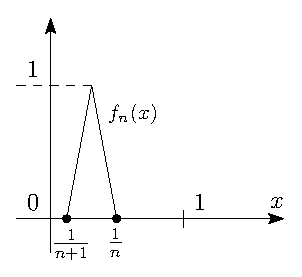
\includegraphics[width=0.3\textwidth]{MA3L10_1.eps}
	\label{10_1}
	\caption{Последовательность функций $f_n(x)$.}
	\label{fig:Равномерная сходимость	}
\end{figure}
Если рассмотрим точную верхнюю грань:
$$
	\sup\limits_{x \in X}|f_n(x) - f_m(x)| = 1
$$
поскольку они все на разных промежутках отличны от нуля. Очевидно, что $f_n$ и никакая её подпоследовательность не удовлетворяет условию Коши $\Rightarrow$ никакая подпоследовательность не может быть сходящейся равномерно, при этом эта последовательность равномерна ограниченна.

Получается, что условия теоремы Больцано нет. Но надо помнить, что 	теорема Больцано связана не только с возможностью выбирать из ограниченного сходящееся, но с компактностью.

\textbf{Причина}: ограниченное замкнутое множество может не быть компактом, потому что для точек компакта было утверждение о том, что если задана последовательность из неё можно выбрать сходяющуюся подпоследовательность. Причина отуствия теоремы Больцано в первую очередь связана с отсутствием компактности ограниченных замкнутых множеств. 

\newpage
\section*{Компактность}
Появляется естественный вопрос, какие множества будут компактами? Можно ли как-то описать компактность? Попробуем разобраться. Нас будут интересовать пространства ограниченных функций: 
$$
	\MB(X) = \{f \colon X \to \MR,\, \sup\limits_{X}|f| <  \infty \}
$$ 
это метрическое пространство с метрикой $\rho(f,g) = \sup\limits_{X}|f - g|$ и соответственно:
$$
	f_n \uconv{X}f \Leftrightarrow \rho(f_n,f) \to 0
$$
по определению равномерной сходимости (взятое из сходимости по метрике). Вопрос, а как устроены компакты в $\MB(X)$? Хочется получить что-нибудь аналогичное конечномерным пространствам, где компакты это ограниченные и замкнутые множества.

\begin{defn}
	Множество $K$ в метрическом пространстве $(X,\rho)$ \uwave{компактно}, если всякое его покрытие открытыми множествами имеет конечное подпокрытие.
\end{defn}

\begin{prop}
	Множество $K \subset \MB(X)$ - компакт, тогда (в неметрическом пространстве это утверждение неверно):
	\begin{enumerate} [label ={\arabic*)}]
		\item $K$ - ограниченное множество;
		\item $K$ - замкнутое множество (дополнение к нему - открыто);
		\item Замкнутое подмножество компакта является компактом;
		\item Всякое бесконечное подмножество обязательно имеет предельную точку;
	\end{enumerate}
\end{prop}
\begin{rem}
	В частности, $4)$ свойство означает, что у всякой последовательности элементов компакта есть сходящаяся подпоследовательность.
\end{rem}
Для продолжения обсуждения, нам потребуется понятие $\VE$-сети.

\begin{defn}
	Пусть $\VE > 0$ и $A$ - подмножество метрического пространства $(X,\rho)$. Множество $B$ называется $\VE$-\uwave{сетью для множества} $A$, если:
	$$
		\forall a \in A, \, \exists \, b \in B \colon \rho(a,b) < \VE
	$$
\end{defn}
\begin{rem}
	То есть, если возьмем множество $B$ и в каждой его точке нарисуем шарик радиуса $\VE$, то эти шары закроют множество $A$.
	\begin{figure}[H]
		\centering
		\includegraphics[width=0.25\textwidth]{MA3L10_2.eps}
		\label{10_2}
		\caption{Покрытие $\VE$ - сетью.}
		\label{fig:Покрытие	}
	\end{figure}
\end{rem}
\begin{rem}
	В общем случае, компактность в метрических пространствах связана не с ограниченностью, а с возможностью поймать множество в такую сеть.
\end{rem}
\begin{defn}
	Если множество $B$ выше конечное, то говорят, что $A$ имеет \uwave{конечную} $\VE$-\uwave{сеть}.	
\end{defn}

\begin{prop}
	Если у множества $A$ есть конечная $\VE$-сеть, то у $A$ есть конечная $2\VE$-сеть из элементов $A$.
\end{prop}
\begin{proof}
	Пусть $B$ это $\VE$-сеть для $A$. Возьмем $b \in B$, если $B(b,\VE) \cap A \neq \VN$, то выбираем $\tilde{a} \in B(b,\VE) \cap A$ и берем все такие $\tilde{a}$ для каждого $b$ (их конечное число). Если шарик пустой - его можно удалить, он не участвует в образовании $\VE$-сети. Таким образом, получаем $\wte{A} = \{\tilde{a}\}$. Возьмем $c \in \wte{A}$, тогда:
	$$
		\exists \, b \in B \colon \rho(b,c) < \VE \wedge \exists \, \tilde{a} \in \wte{A} \colon \rho(b, \tilde{a}) < \VE \Rightarrow \rho(c, \tilde{a}) < 2\VE
	$$
\end{proof}
\begin{prop}
	Если $K$ - компакт, то у него $\forall \VE > 0$ существует конечная $\VE$-сеть.
\end{prop}
\begin{proof}
	Возьмем $\forall b \in K$ шар $B(b,\VE)$, тогда их объединение покрывает $K$, то есть: 
	$$
		K \subset \bigcup\limits_{b} B(b, \VE)
	$$ 
	Но эти шары открытые $\Rightarrow$ существует конечное подпокрытие: $B(b_1, \VE), \dotsc, B( b_N, \VE)$, по определению компакта. А значит $B = \{b_1, \dotsc, b_N\}$ это и есть конечная $\VE$-сеть.
\end{proof}

\end{document}